
\section{MCS Performance on Truth-Selected Muons from numuCC Events in Simulation}\label{MCBNB_performance_section}


% Executive summary
In this section, studies from this truth-selected simulated BNB numuCC muon sample with {\sc MCTracks} are described. Additionally, similar studies on this sample using automatically reconstructed tracks is described. This section also includes a study justifying that range-based energy is an accurate predictor of true energy for contained muons (with bias less than 1\% and resolution better than 4\%), and therefore can be used in place of true energy so as to compare MC directly to data. The MCS performance on this sample of {\sc MCTracks} is shown to be comparable to that on automatically reconstructed PandoraNuPMA tracks when the track is well reconstructed, with a bias below 5\% and a resolution that varies between 2 and 10\%, performing better for higher momentum (longer) tracks. The resolution is slightly worse for reconstructed tracks than for {\sc MCtracks}. Additionally, the scattering angle of track segments for a given momentum is shown to be similarly gaussian both for {\sc MCTracks} and well reconstructed tracks, in line with the Highland formula prediction.

\subsection{Input Sample}\label{MCBNB_input_sample_section}
The input sample to this portion of the analysis is is 772,000 MCC7 simulated BNB neutrino interactions without any cosmics simulated. These simulated events are run through a fully automated reconstruction chain and then truth information is used to select muons from numuCC interactions which are eligible for MCS analysis. The SAM definition used for this sample is ``prodgenie\_bnb\_nu\_uboone\_mcc7\_reco2''.


\subsection{Fiducial Volume Definition}\label{fidvol_section}
The {\ub} TPC has active volume dimensions of 2.6 m width $\times$ 2.3 m height $\times$ 10.4 m length. For this analysis, a smaller ``fiducial volume'' is defined and referenced throughout this note (for example, in many cases reconstructed tracks are required to be fully contained within the fiducial volume). For reference, the fiducial volume definition used throughout this note is the full TPC volume reduced in by 20 cm from both the cathode plane and the anode wire planes, shifted in 26.5 cm in from both the top and bottom walls of the TPC, shifted in 20 cm from the beam-upstream wall of the TPC, and shifted in 36.8 cm from the downstream wall of the TPC. The reason for this choice of fiducial volume is that it reduces contamination from ``edge effects'' that occur near the walls of the TPC, like electric field distortions and space-charge effects. While the TPC has a total active volume of 62.6 $m^3$, the fiducial volume used in this analysis has a volume of 38.7 $m^3$ or roughly 62\% of the total TPC active volume.









\subsection{Performance with {\sc MCTracks}}\label{MCBNBMCTrack_performance_section}


\subsubsection{MCTrack Description}\label{MCTrack_section}
{\sc MCTrack} objects are made from the output of {\sc geant}4, and are created from {\sc geant}4 energy depositions in the detector. {\sc geant}4 outputs 3D energy depositions in the detector, along with truth information about which parent particles deposited this energy. {\sc MCTracks} are 3D objects which are formed by grouping the energy depositions based on parent particles. Whether a particle in {\sc geant}4 is turned into an {\sc MCTrack} or an {\sc MCShower} (not discussed in this note) is based on truth PDG (for example, muons, protons, and pions always form {\sc MCTracks}).\\

Each {\sc MCTrack} is itself a vector of 3D trajectory points, which are ordered to match the direction of the particle that deposited the energy. Trajectory points are only formed for energy depositions inside of the TPC volume. In general, long {\sc MCTrack}s will have steps separated by up to several centimeters. Each step in an {\sc MCTrack} holds the following information used in this analysis: 3D position, and true energy at that point. Only information within the realm of reconstructable quantities is used in this analysis, with the exception of true energy (which is used for example to quantify a reconstructed energy resolution).\\

Since the output of a nominal reconstruction chain (including hit finding, clustering, matching across planes, etc.) are 3D tracks, {\sc MCTracks} can be studied in an analysis in the exact same way as a reconstructed track would be. {\sc MCTracks} can be thought of as perfectly reconstructed tracks, where each trajectory point along the track is a true 3D energy deposition inside of the {\ub} TPC.\\

Since {\sc MCTracks} are formed from true 3D energy depositions and not from wire signals on drift electrons, {\sc MCTracks} are insensitive to broken wires, noise, and other simulated detector effects.\\

It is worth noting that delta rays eminating from muon tracks are relevant for MCS calculations. Here, delta rays form {\sc MCShowers} and are therefore invisible to this analysis. This is the same as assuming the reconstructed tracks have perfectly removed charge from delta rays in their algorithms.




\subsubsection{Event Selection}\label{MCBNBMCTrack_eventselection_section}
The event selection for this subanalysis is truth based. The fiducial volume used in this subanalysis is the same as is used throughout the note, defined in Section \ref{fidvol_section}. Beginning with the 772,000 events in the sample, the cuts placed are:

\begin{itemize}
\item There is one neutrino interaction in the event (770,241 events remain).
\item The neutrino interaction is of type charged-current (559,348 events remain).
\item The neutrino interaction occurs within the fiducial volume (152,214 events remain).
\item The interacting neutrino is type $\nu_\mu$ (149,684 events remain).
\item The {\sc MCTrack} associated with the outgoing muon from the interaction is fully contained within the fiducial volume (50,537 events remain).
\item The {\sc MCTrack} associated with the outgoing muon from the interaction is at least one meter in length (23,378 events remain).
\item The {\sc MCTrack} associated with the outgoing muon from the interaction does not decay in flight (this cut is implemented by requiring the {\sc MCTrack}'s total energy at its final trajectory point is equal to the muon mass) (23,342 events remain).
\end{itemize}
After these additional cuts are placed, 23342 events ({\sc MCTracks}) remain for MCS analysis. The energy and angle distributions for these 23342 muons can be seen in Figure \ref{BNBmuon_energy_angle_fig}. It should be noted that any computed metrics from this sample (and therefore any other BNB sample) have convolved any effects of performance differences as a function of angle.\\

\begin{figure}
\centering
\mbox{
	\subfigure[\textit{Muon energy distribution.}]
	{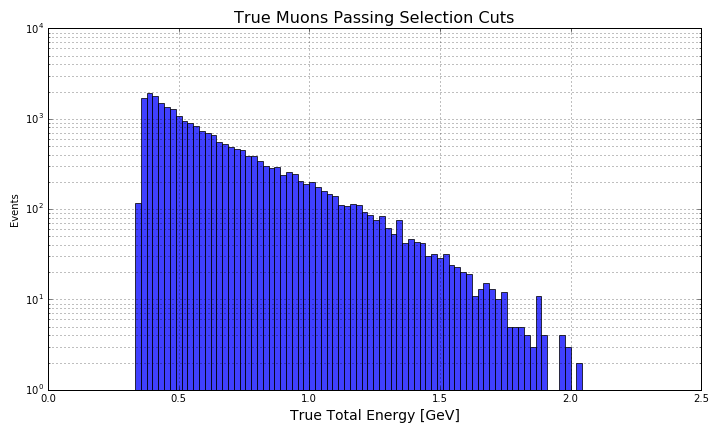
\includegraphics[width=75mm]{Figures/MCBNBMCTrack_EnergySpectrum.png}}
	\quad
	\subfigure[\textit{Muon theta angle (angle with respect to the beam direction) distribution.}]
	{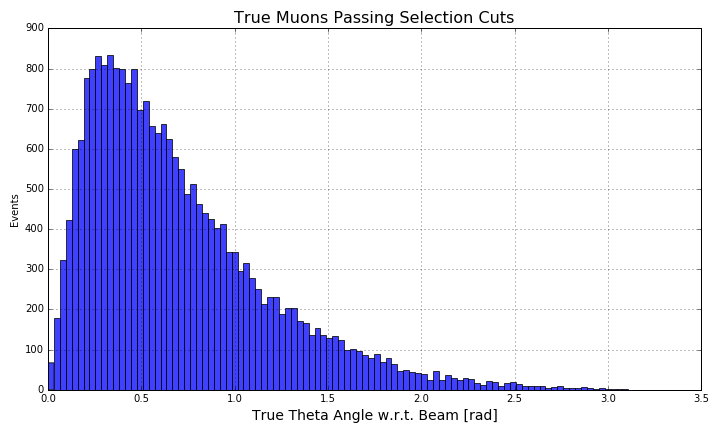
\includegraphics[width=75mm]{Figures/MCBNBMCTrack_AngleSpectrum.png}}
	}
\caption{\textit{Energy and angle distributions for muons from numuCC interactions in {\ub} simulation passing cuts described in Section \ref{MCBNBMCTrack_eventselection_section}.}}
\label{BNBmuon_energy_angle_fig}
\end{figure}



\subsubsection{Range Energy Validation}\label{Range_Energy_Validation_section}
With this sample of {\sc MCTracks}, it is possible to quantify MCS energy (momentum) resolution as a function of true energy (momentum). However, in actual {\ub} data there is obviously no true momentum with which to compare. The additional momentum handle that is used in data for contained tracks is range-based energy. The stopping power of muons in liquid argon is well described by the particle data group\cite{PDG_spline_table}. By using a linear interpolation between points in the cited PDG stopping power table, the start-to-end straight-line length of a track can be used to reconstruct the muon's total energy with good accuracy. Figure \ref{true_range_energy_MCTrack_fig} shows a comparison of range energy to true energy for this sample. \\

In order to compute a bias and a resolution, Figure \ref{true_range_energy_MCTrack_fig} is sliced in bins of true muon energy and a histogram of the fractional energy difference ($\frac{E_{range} - E_{true}}{E_{true}}$) is created for each bin. This distribution is shown for three representative bins in Figure \ref{true_range_bias_resolution_MCTrack_slices_fig}, along with the gaussian fit to each.  The mean ($\mu$) of each gaussian fit is used to compute a bias as a function of true energy, while the width ($\sigma$) of each distribution is used to compute a resolution. Figure \ref{true_range_bias_resolution_MCTrack_fig} shows the bias and resolution for the range-based energy reconstruction method. It can be seen that the bias is negligible and the resolution for this method of energy reconstruction is on the order of 2-4\%. Based on this figure, it is clear that range-based energy (and therefore range-based momentum) is a good handle on the true energy (momentum) of a reconstructed muon track in {\ub} data, assuming that track is well reconstructed in terms of length.

\begin{figure}[ht!]
\begin{center}
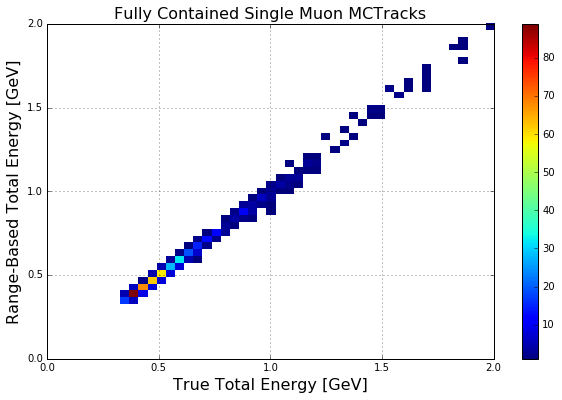
\includegraphics[width=100mm]{Figures/true_range_comparison_MCTracks.png}
\end{center}
\caption{\textit{Range based energy versus true energy for the {\sc MCTrack} sample described in Section \ref{MCBNBMCTrack_eventselection_section}.}}
\label{true_range_energy_MCTrack_fig}
\end{figure}

\begin{figure}
\centering
\mbox{
	\subfigure[\textit{Fractional energy difference between 0.35 and 0.53 GeV true energy.}]
	{\includegraphics[width=50mm]{Figures/{true_range_resolution_MCBNBMCTrack_slice_0.35_0.53}.png}}
	\quad
	\subfigure[\textit{Fractional energy difference between 0.90 and 1.08 GeV true energy.}]
	{\includegraphics[width=50mm]{Figures/{true_range_resolution_MCBNBMCTrack_slice_0.90_1.08}.png}}
	\quad
	\subfigure[\textit{Fractional energy difference between 1.45 and 1.63 GeV true energy.}]
	{\includegraphics[width=50mm]{Figures/{true_range_resolution_MCBNBMCTrack_slice_1.45_1.63}.png}}
	}
\caption{\textit{Fractional energy difference for a few representative bins of true energy derived from Figure \ref{true_range_energy_MCTrack_fig}.}}
\label{true_range_bias_resolution_MCTrack_slices_fig}
\end{figure}




\begin{figure}
\centering
\mbox{
	\subfigure[\textit{Range energy bias as a function of true energy. The vertical error bars are computed as $\frac{\sigma_{fit}}{\sqrt{N}}$, and the horizontal error bars indicate bin width.}]
	{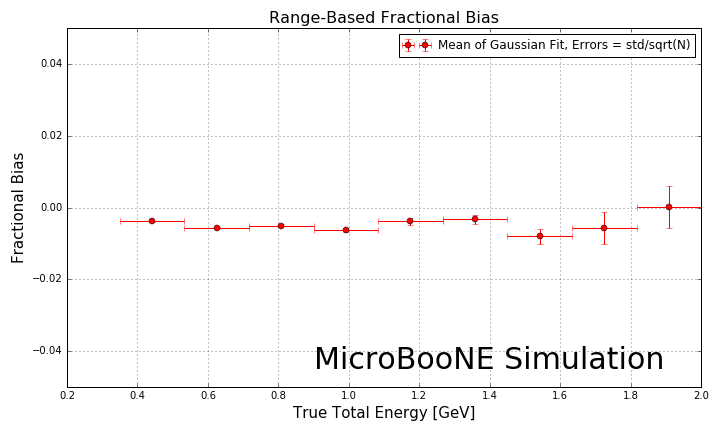
\includegraphics[width=75mm]{Figures/true_range_bias_MCBNBMCTrack.png}}
	\quad
	\subfigure[\textit{Range energy resolution as a function of true energy. The vertical error bars are computed as $\frac{\sigma_{fit}}{\sqrt{2N}}$, and the horizontal error bars indicate bin width.}]
	{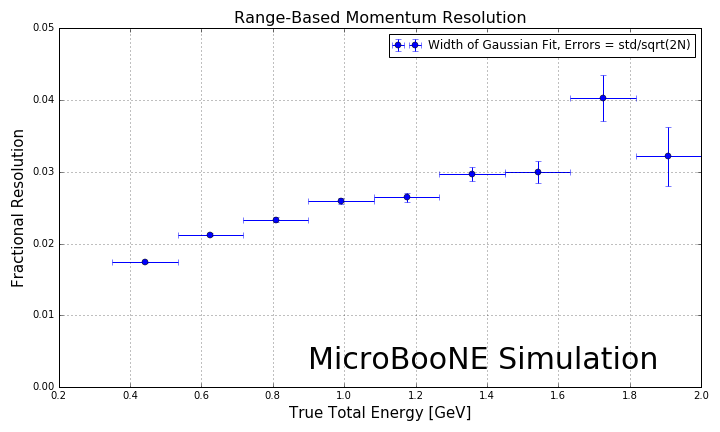
\includegraphics[width=75mm]{Figures/true_range_resolution_MCBNBMCTrack.png}}
	}
\caption{\textit{Range energy and true energy bias and resolution for the {\sc MCTrack} sample described in Section \ref{MCBNBMCTrack_eventselection_section}.}}
\label{true_range_bias_resolution_MCTrack_fig}
\end{figure}







\subsubsection{MCS Momentum Validation}\label{MCS_Momentum_Validation_MCTrack_section}
For this sample of {\sc MCTracks}, only the 3D trajectory points of each {\sc MCTrack} are used as input to the MCS code, described in Section \ref{MCS_technique_section}. The resulting MCS momentum versus range-based momentum can be seen in Figure \ref{MCS_range_momentum_MCTrack_fig}. Range momentum is used here instead of true momentum in order to make this plot more directly comparable with the same analysis on data where true momentum is not accessible. In order to compute a bias and a resolution, Figure \ref{MCS_range_momentum_MCTrack_fig} is sliced in bins of range momentum and a histogram of the fractional momentum difference ($\frac{p_{MCS}^{-1} - p_{range}^{-1}}{p_{range}^{-1}}$) is created for each bin\footnote{The choice of using inverse momentum is justified in Appendix \ref{inverse_p_justification_section}.}. This distribution is shown for three representative bins in Figure \ref{MCS_range_bias_resolution_MCTrack_slices_fig}, along with the gaussian fit to each.  The mean ($\mu$) of each gaussian fit is used to compute a bias as a function of range momentum, while the width ($\sigma$) of each distribution is used to compute a resolution. The bias and resolution for this momentum reconstruction method shown in Figure \ref{MCS_range_bias_resolution_MCTrack_fig}. This figure indicates a bias in the MCS momentum resolution on the order of a few percent, with a resolution that decreases from about 9\% for contained {\sc MCTracks} with true total momentum around 0.5 GeV (which corresponds to a length of about 1.7 meters) to below 3\% for contained {\sc MCTracks} with true total momentum greater than 0.8 GeV (which corresponds to a length of about 3.1 meters).


\begin{figure}[ht!]
\begin{center}
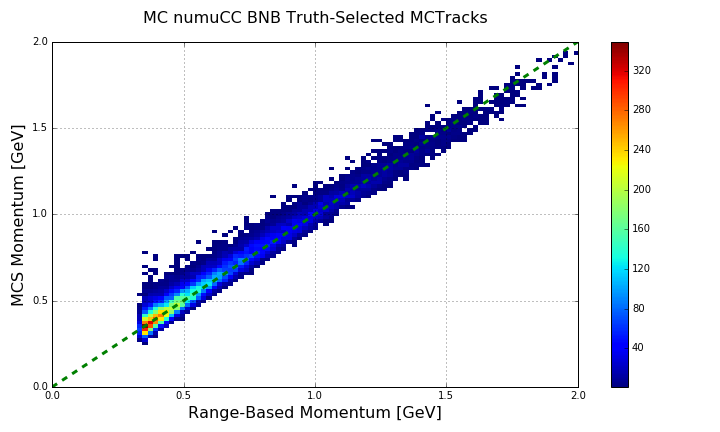
\includegraphics[width=100mm]{Figures/MCS_range_comparison_MCBNBMCTrack.png}
\end{center}
\caption{\textit{MCS computed momentum versus range momentum for the {\sc MCTrack} sample described in Section \ref{MCBNBMCTrack_eventselection_section}. Note the cutoff at around 0.3 GeV range-based momentum is caused by the minimum track length of 100 centimenter requirement.}}
\label{MCS_range_momentum_MCTrack_fig}
\end{figure}

\begin{figure}
\centering
\mbox{
	\subfigure[\textit{Fractional momentum difference between 0.35 and 0.53 GeV range momentum.}]
	{\includegraphics[width=50mm]{Figures/{MCS_range_resolution_MCBNBMCTrack_slice_0.35_0.53}.png}}
	\quad
	\subfigure[\textit{Fractional momentum difference between 0.90 and 1.08 GeV true momentum.}]
	{\includegraphics[width=50mm]{Figures/{MCS_range_resolution_MCBNBMCTrack_slice_0.90_1.08}.png}}
	\quad
	\subfigure[\textit{Fractional momentum difference between 1.45 and 1.63 GeV true momentum.}]
	{\includegraphics[width=50mm]{Figures/{MCS_range_resolution_MCBNBMCTrack_slice_1.45_1.63}.png}}
	}
\caption{\textit{Fractional momentum difference for a few representative bins of range momentum derived from Figure \ref{MCS_range_momentum_MCTrack_fig}.}}
\label{MCS_range_bias_resolution_MCTrack_slices_fig}
\end{figure}


\begin{figure}
\centering
\mbox{
	\subfigure[\textit{MCS momentum bias as a function of range momentum. The vertical error bars are computed as $\frac{\sigma_{fit}}{\sqrt{N}}$, and the horizontal error bars indicate bin width.}]
	{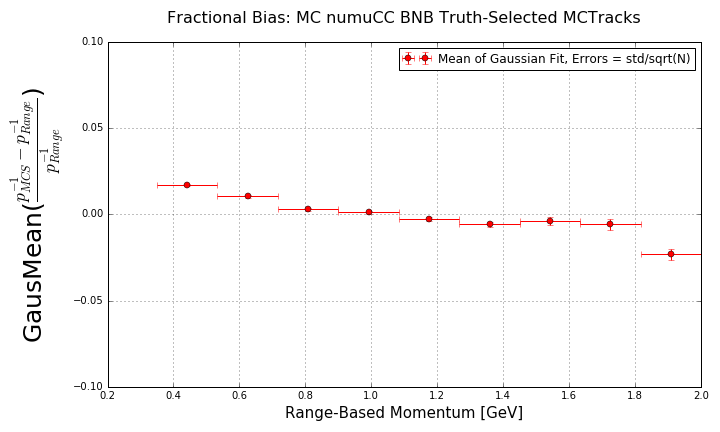
\includegraphics[width=75mm]{Figures/MCS_range_bias_MCBNBMCTrack.png}}
	\quad
	\subfigure[\textit{MCS momentum resolution as a function of range momentum. The vertical error bars are computed as $\frac{\sigma_{fit}}{\sqrt{2N}}$, and the horizontal error bars indicate bin width.}]
	{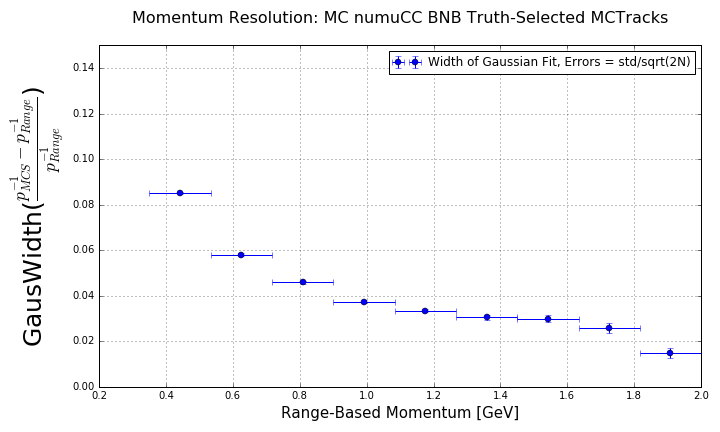
\includegraphics[width=75mm]{Figures/MCS_range_resolution_MCBNBMCTrack.png}}
	}
\caption{\textit{MCS momentum bias and resolution as a function of range momentum for the {\sc MCTrack} sample described in Section \ref{MCBNBMCTrack_eventselection_section}.}}
\label{MCS_range_bias_resolution_MCTrack_fig}
\end{figure}



\subsubsection{Highland Validation}\label{Highland_Validation_MCTrack_section}
For a given track segment momentum and length, 98\% of the angular scatter deviations should be gaussian with an RMS described by the Highland equation (Equation \ref{highland_eqtn}), while the remaining 2\% are larger angle Rutherford scatters\cite{highland}\footnote{This is not actually taken into account explicitly in the current algorithm implementation}. Therefore, a histogram of track segment angular deviations divided by the RMS predicted by the Highland equation should be gaussian with a width of unity. In this section, we validate this claim.\\

For each 10 cm segment of each {\sc MCTrack} in this single muon sample, the momentum of the muon at the start of that segment is estimated by taking the computed MCS momentum and subtracting out momentum lost in the track upstream of the start of this segment, assuming the track was minimally ionizing as described in Equation \ref{segment_E_equation}. The segment momentum, along with the segment length, is converted into an expected RMS angular deviation by way of Equation \ref{highland_eqtn}. For each consecutive pair of segments, the angular scatter in milliradians divided by the Highland expected RMS in millradians is an entry in the histogram shown in Figure \ref{Highland_validation_MCTracks_fig}. From this figure we can see that the Highland formula is valid for {\sc MCTracks}, as the gaussian fit agrees well with the underlying histogram.

\begin{figure}[ht!]
\begin{center}
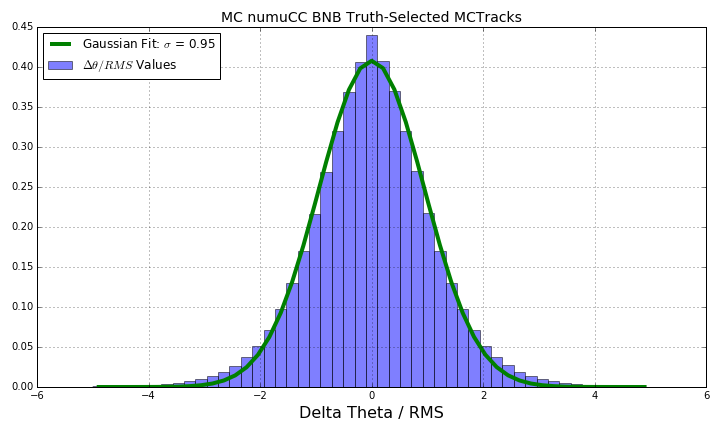
\includegraphics[width=100mm]{Figures/Highland_validation_MCBNBMCTrack.png}
\end{center}
\caption{\textit{10 cm segment angular deviations divided by expected Highland RMS for the single muon {\sc MCTrack} sample described in Section \ref{MCBNBMCTrack_eventselection_section}.}}
\label{Highland_validation_MCTracks_fig}
\end{figure}




























\subsection{Performance with Reconstructed Tracks}\label{MCBNBRecoTrack_performance_section}

\subsubsection{Event Selection}\label{MCBNBRecoTrack_eventselection_section}
The event selection for this subanalysis is identical to that described in Section \ref{MCBNBMCTrack_eventselection_section} with one additional cut. The additional cut is requiring that there is a reconstructed track which starts within 3 cm of the start and ends within 3 cm of the end of the aforementioned {\sc MCTrack} (or vice-versa). This cut is requiring that the track is well reconstructed in terms of position (direction is taken into account later). 13810 events pass this cut, down from the 23342 previously.

\subsubsection{MCS Momentum Validation}\label{MCS_Momentum_Validation_MCBNBRecoTrack_section}
For this sample of reconstructed tracks, only the 3D trajectory points of each reconstructed track are used as input to the MCS code, described in Section \ref{MCS_technique_section}. The resulting MCS momentum versus range-based momentum for this sample of reconstructed tracks without any cuts other than those described in Section \ref{MCBNBRecoTrack_eventselection_section} can be seen in Figure \ref{MCS_range_momentum_MCBNBRecoTrack_fig}. \\

In order to compute a bias and a resolution, Figure \ref{MCS_range_momentum_MCBNBRecoTrack_fig} is sliced in bins of range momentum and a histogram of the fractional momentum difference ($\frac{p_{MCS}^{-1} - p_{range}^{-1}}{p_{range}^{-1}}$) is created for each bin\footnote{The choice of using inverse momentum is justified in Appendix \ref{inverse_p_justification_section}}. This distribution is shown for three representative bins in Figure \ref{MCS_range_bias_resolution_MCBNBRecoTrack_slices_fig}, along with the gaussian fit to each.  The mean ($\mu$) of each gaussian fit is used to compute a bias as a function of range momentum, while the width ($\sigma$) of each distribution is used to compute a resolution. The bias and resolution for this momentum reconstruction method shown in Figure \ref{MCS_range_bias_resolution_MCBNBRecoTrack_fig}. This figure indicates a bias in the MCS momentum resolution on the order of a few percent, with a resolution that decreases from about 9\% for contained tracks with true total momentum around 0.5 GeV (which corresponds to a length of about 1.7 meters) to below 7\% for contained tracks with true total momentum greater than 0.8 GeV (which corresponds to a length of about 3.1 meters). This agrees reasonably well with the analogous plots created from simulated single muons with {\sc MCTracks} (Figure \ref{MCS_range_bias_resolution_MCTrack_fig}).


\begin{figure}[ht!]
\begin{center}
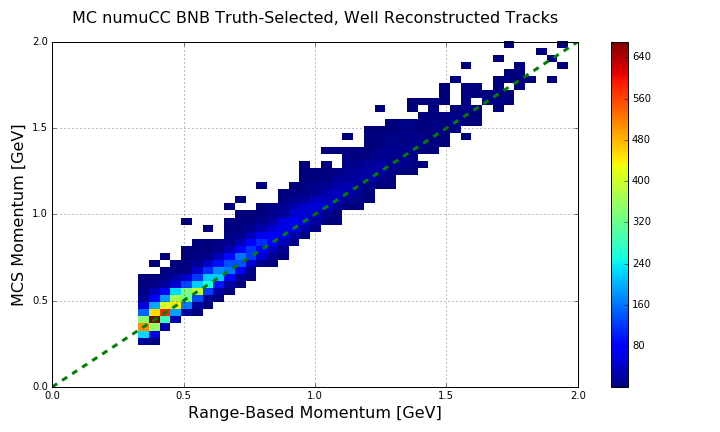
\includegraphics[width=100mm]{Figures/MCS_range_comparison_MCBNBRecoTrack.png}
\end{center}
\caption{\textit{MCS computed momentum versus range momentum for the truth-selected simulated fully contained, well reconstructed muon tracks from numu charged current events.}}
\label{MCS_range_momentum_MCBNBRecoTrack_fig}
\end{figure}


\begin{figure}
\centering
\mbox{
	\subfigure[\textit{Fractional momentum difference between 0.35 and 0.53 GeV range momentum.}]
	{\includegraphics[width=50mm]{Figures/{MCS_range_resolution_MCBNBRecoTrack_slice_0.35_0.53}.png}}
	\quad
	\subfigure[\textit{Fractional momentum difference between 0.90 and 1.08 GeV range momentum.}]
	{\includegraphics[width=50mm]{Figures/{MCS_range_resolution_MCBNBRecoTrack_slice_0.90_1.08}.png}}
	\quad
	\subfigure[\textit{Fractional momentum difference between 1.45 and 1.63 GeV range momentum.}]
	{\includegraphics[width=50mm]{Figures/{MCS_range_resolution_MCBNBRecoTrack_slice_1.45_1.63}.png}}
	}

\caption{\textit{Fractional momentum difference for a few representative bins of range momentum derived from Figure \ref{MCS_range_momentum_MCBNBRecoTrack_fig}.}}
\label{MCS_range_bias_resolution_MCBNBRecoTrack_slices_fig}
\end{figure}


\begin{figure}
\centering
\mbox{
	\subfigure[\textit{MCS momentum bias as a function of range momentum. The vertical error bars are computed as $\frac{\sigma_{fit}}{\sqrt{N}}$, and the horizontal error bars indicate bin width.}]
	{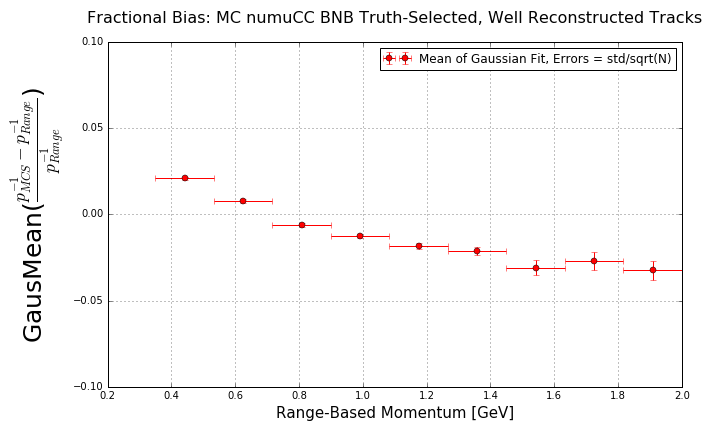
\includegraphics[width=75mm]{Figures/MCS_range_bias_MCBNBRecoTrack.png}}
	\quad
	\subfigure[\textit{MCS momentum resolution as a function of range momentum. The vertical error bars are computed as $\frac{\sigma_{fit}}{\sqrt{2N}}$, and the horizontal error bars indicate bin width.}]
	{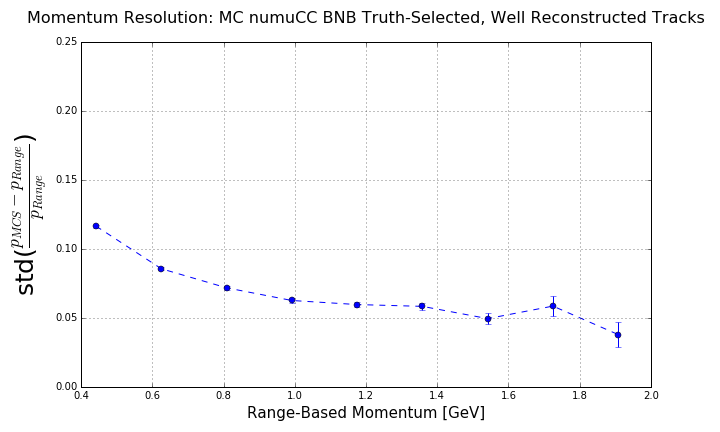
\includegraphics[width=75mm]{Figures/MCS_range_resolution_MCBNBRecoTrack.png}}
	}
\caption{\textit{MCS momentum bias and resolution as a function of range momentum for the truth-selected simulated fully contained, well reconstructed muon tracks from numu charged current events.}}
\label{MCS_range_bias_resolution_MCBNBRecoTrack_fig}
\end{figure}



\subsubsection{Highland Validation}\label{Highland_Validation_MCBNBRecoTrack_section}
For this sample of tracks, the same Highland validation plot is created in exactly the same way as described in Section \ref{Highland_Validation_MCTrack_section}. For each consecutive pair of segments, the angular scatter in milliradians divided by the Highland expected RMS in millradians is an entry in the histogram shown in Figure \ref{Highland_validation_MCBNBRecoTrack_fig}. From this figure we can see that the Highland formula is valid for well reconstructed tracks in simulation when 10 cm segments are used.

\begin{figure}[ht!]
\begin{center}
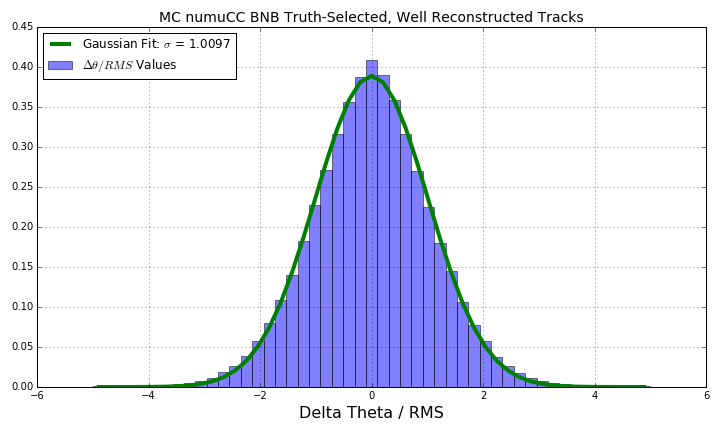
\includegraphics[width=100mm]{Figures/Highland_validation_MCBNBRecoTrack.png}
\end{center}
\caption{\textit{10 cm segment angular deviations divided by expected Highland RMS for the sample of well reconstructed, neutrino induced muons in simulation.}}
\label{Highland_validation_MCBNBRecoTrack_fig}
\end{figure}



